\documentclass[11pt]{article}
\usepackage[T1]{fontenc}
\usepackage[utf8]{inputenc}
\usepackage{lmodern,amsmath,amssymb,graphicx,geometry,microtype,setspace,booktabs,caption}
\usepackage[hidelinks]{hyperref}
\geometry{letterpaper,margin=1in}
\setlength{\parindent}{0pt}
\setlength{\parskip}{0.55em}
\setlength{\emergencystretch}{2em}
\captionsetup{labelfont=bf,font=small}
\renewcommand{\refname}{References}

\pagestyle{empty}
\renewcommand{\thefigure}{S\arabic{figure}}
\setcounter{figure}{8}

\begin{document}
\begin{figure}[!ht]\centering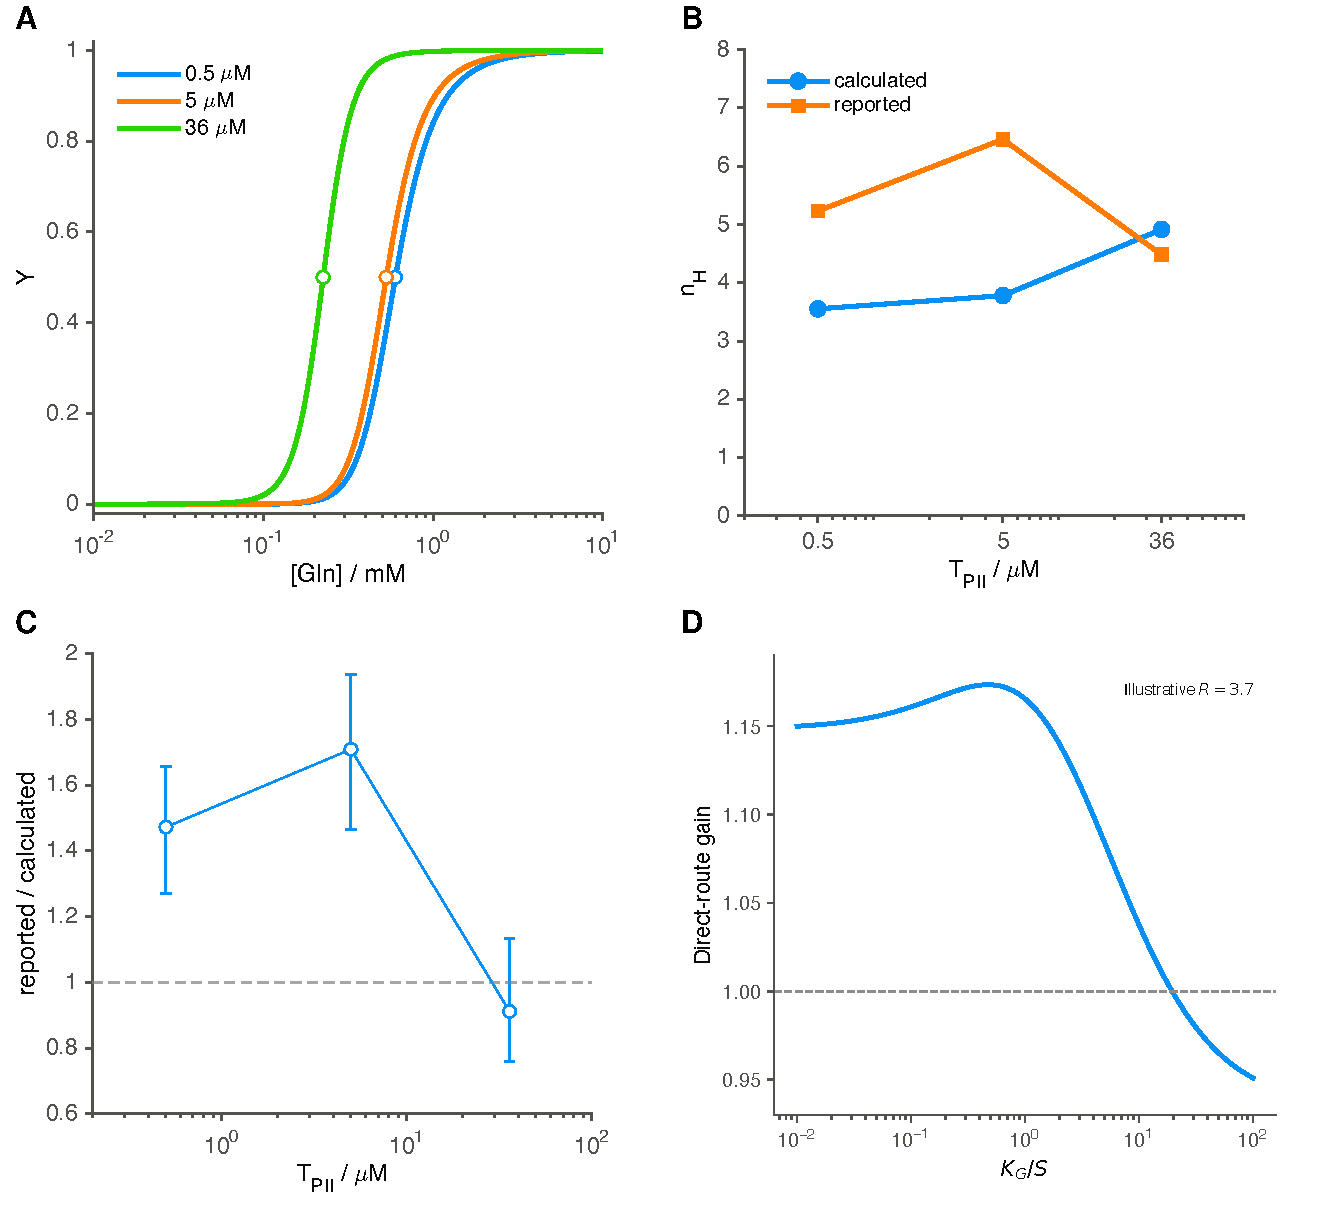
\includegraphics[width=\textwidth,height=0.62\textheight,keepaspectratio]{figure_inputs/FigS9_baseline.pdf}\begin{singlespace}\caption{\textbf{Conditional accounting of cascade sensitivity and a direct glutamine route.} (A) Calculated downstream responses normalized between their limiting plateaus. Points mark calibrated reported midpoints; curves are model outputs, not experimental traces. (B) Calculated response-range coefficients and reported cascade coefficients at three PII concentrations. PII concentrations of 0.5, 5, and 36 micromolar correspond to UTase/UR concentrations of 0.05, 0.5, and 0.8 micromolar. (C) Ratios of reported to calculated coefficients. Error bars span central 95\% ranges from upstream coordinate perturbations only; connected points aid reading and do not establish a non-monotonic mechanism. (D) Gain produced by the illustrative direct activation law with R=3.7 while retaining the downstream scale calibrated before adding the route. The gain spans approximately 0.95--1.17 and does not supply the middle-condition discrepancy in this specified construction.}\end{singlespace}\end{figure}
\end{document}
